\section{Theorie}
\label{sec:Theorie}
Ein Lock-In-Verstärker besteht prinzipiell aus einem Bandpassfilter, .... Dieser schematische Aufbau ist in \autoref{fig:schema} dargestellt.
\begin{figure}[H]
    \centering
    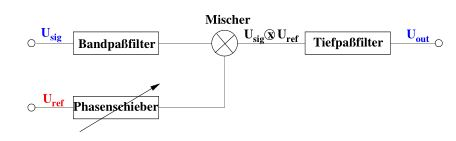
\includegraphics{images/schema.JPG}
    \caption{Schematischer Aufbau eines Lock-In-Verstärkers\cite{sample}}
    \label{fig:schema}
\end{figure}
\noindent